\documentclass{standalone}
\usepackage{tikz}
\usetikzlibrary{calc}

\begin{document}
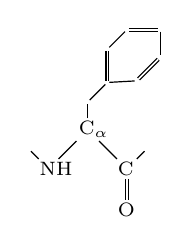
\begin{tikzpicture}
    % implicit atoms (C)
    \tikzstyle{imp}=[inner sep=0, font=\scriptsize, text width=0ex]
    % explicit atoms with name
    \tikzstyle{exp}=[inner sep=1, font=\scriptsize, text width=1.5ex]
    \node[exp] (NH) at (0,0) {NH};
    \node[exp] (CA) at ($(NH)+(45:2em)$) {C$_{\alpha}$};
    \node[exp] (CO) at ($(CA)+(-45:2em)$) {C};
    \node[exp] (O) at ($(CO)+(90:-1.5em)$) {O};
    \node[imp] (CB) at ($(CA)+(90:1.em)$) {};
    \node[imp] (CG) at ($(CB)+(45:1.em)$) {};
    \node[imp] (CD1) at ($(CG)+(90:1.2em)$) {};
    \node[imp] (CE1) at ($(CD1)+(45:1.em)$) {};
    \node[imp] (CZ) at ($(CE1)+(0:1.2em)$) {};
    \node[imp] (CE2) at ($(CZ)+(-90:1.em)$) {};
    \node[imp] (CD2) at ($(CE2)+(-135:1.2em)$) {};
    \node[imp] (DUM0) at ($(NH)+(-45:-1.em)$) {};
    \node[imp] (DUM1) at ($(CO)+(45:1.em)$) {};
    \draw[line width=.1ex] (DUM0) -- (NH) -- (CA) -- (CO) -- (DUM1);
    \draw[line width=.1ex, double] (CO) -- (O);
    \draw[line width=.1ex] (CA) -- (CB);
    \draw[line width=.1ex] (CB) -- (CG);
    \draw[line width=.1ex, double] (CG) -- (CD1);
    \draw[line width=.1ex] (CD1) -- (CE1);
    \draw[line width=.1ex, double] (CE1) -- (CZ);
    \draw[line width=.1ex] (CZ) -- (CE2);
    \draw[line width=.1ex, double] (CE2) -- (CD2);
    \draw[line width=.1ex] (CD2) -- (CG);
\end{tikzpicture}
\end{document}
